\documentclass[letterpaper,11pt]{article}

\usepackage{graphicx}
\usepackage{multicol}
\usepackage{fullpage}
\usepackage{csquotes}
\usepackage[margin=0.75in,letterpaper]{geometry}
\setlength{\footskip}{15pt}
\setlength{\belowcaptionskip}{9pt}
\usepackage{floatflt}
\usepackage{xspace}
\usepackage[margin=1cm,skip=9pt]{caption}
\usepackage{ulem}
\usepackage{tikz}
\usetikzlibrary{shadows}

% https://tex.stackexchange.com/questions/5226/keyboard-font-for-latex
\newcommand*\keys[1]{%
  \tikz[baseline=(key.base)]
    \node[%
      draw,
      fill=white,
      drop shadow={shadow xshift=0.25ex,shadow yshift=-0.25ex,fill=black,opacity=0.75},
      rectangle,
      rounded corners=2pt,
      inner sep=1pt,
      line width=0.5pt,
      minimum width=1.1em,
      font=\scriptsize\sffamily
    ](key) {#1\strut}
  ;
}

\linespread{0.95}
\def\degC{$^{\circ}$C }
\def\degf{$^{\circ}$F }
\def\vol #1 {{\bf #1}, $\;\;$}
\def\refer{\par\noindent\hangindent\parindent\hangafter1}


\title{\vspace{-2.0cm}Herzmann Family Christmas Letter 2020}
\author{Daryl Herzmann${}^1$, Elizabeth Herzmann${}^2$, Margaret 
Herzmann${}^3$,\\
Robert Herzmann${}^4$, AND Charlotte Herzmann${}^5$ \\
\it{${}^1$Mellifluous Author},
\it{${}^2$Responsible Adult},
\it{${}^3$Fledgling Dancer},
\it{${}^4$Runt-Runt},
\it{${}^5$Almost Four!}}
\date{17 December 2020}

\makeatletter
\newenvironment{tablehere}
  {\def\@captype{table}}
  {}

\newenvironment{figurehere}
  {\def\@captype{figure}}
  {}
\makeatother

\newcommand{\Line}[0]{%
  \rule{0cm}{0cm}\\\hrule\rule{0cm}{0cm}%
}

%\addtolength{\textheight}{1.5in}

\begin{document}
\maketitle
\vspace{-0.75cm}
\begin{abstract}
Our seminal 2018 Christmas Letter (Herzmann et al., 2018) first attributed the passage
of another year's worth of time to attrition.  The same was not to be true for the
year 2020.  This letter summarizes our fortunate year of surviving \textit{COVID-19},
the derecho of 10 August 2020, virtual schooling, and the presidential election.
\end{abstract}

\vspace{-0.5cm}

\noindent\makebox[\linewidth]{\rule{\textwidth}{1pt}}

\begin{multicols}{2}

\section{Introduction} 

The size of our family is unchanged this year and comprises Daryl
\enquote{Daryl} (42), Elizabeth \enquote{Liz} (28+),
Margaret \enquote{Maggie Moo} (7), Robert \enquote{Ro-Ro} (6), Charlotte
 \enquote{Charly Friend} (3), and one cat with a dog's name of Snoopy (12). 
We are thankful to have survived the various calamities of 2020 and the
children from each other.
   
\subsection{Housing}

Our lone house has not moved and thankfully survived the 15 minutes of 
70-80 MPH ($\approx$ 35 $m s^{-1}$)
wind gusts during the August derecho.  Our lone tree was shielded by the house
and was not damaged. The only damage is shown by Figure 1 with
the cheap charcoal grill busting out a side of a poorly constructed deck.
The immediate lesson learned was to acquire a propane grill (Hill, 2003).

\bigskip

\begin{figurehere}
    \centering   
    \resizebox{.95\columnwidth}{!}{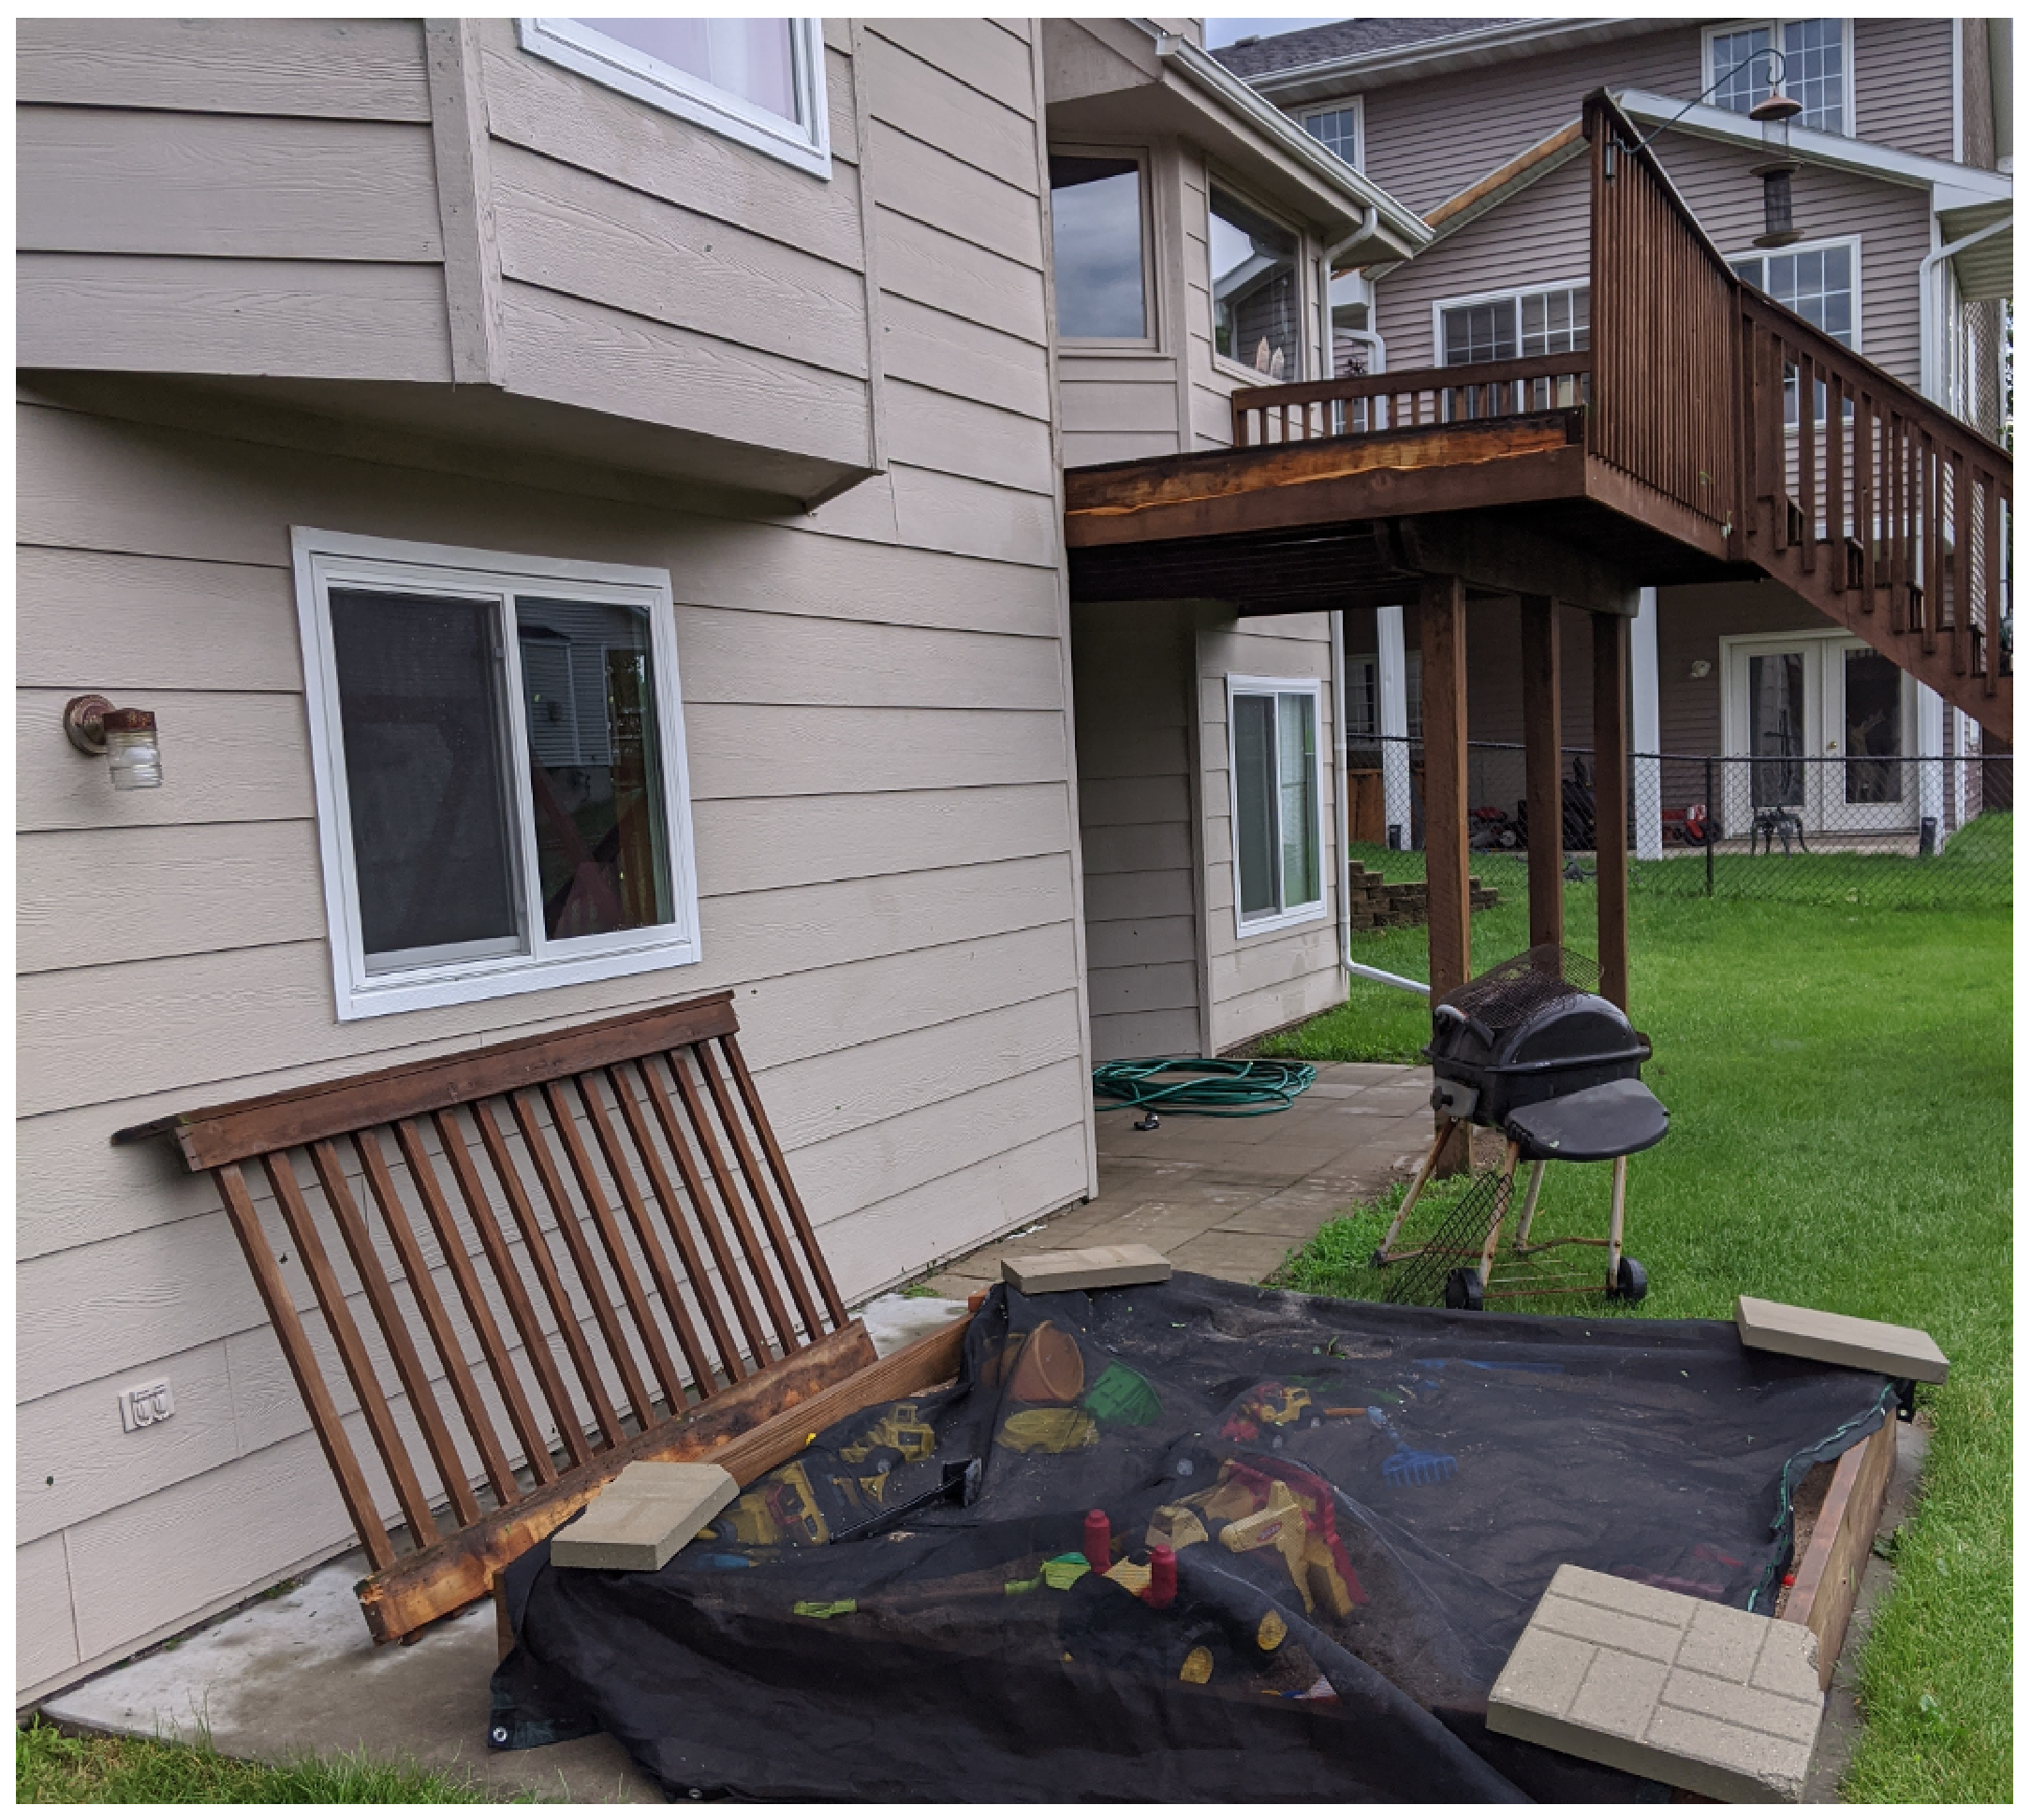
\includegraphics[angle=0]{plots/f1_2020.eps}}
    \caption{We will rebuild and have already rebuilt with screws this time.}
\end{figurehere}

To buoy the economy, we decided to effort a large number of remodeling projects
around the house. We a) replaced the roof, b) replaced six exterior doors and
windows (Figure 2), c) replaced kid destroyed dining room carpet with plank, d) replaced 
kitchen peninsula with an island and e) Daryl finally got a broken kitchen cabinet
fixed after eight years of supposed diligent home ownership.

\subsection{Employment}

Daryl is somehow still employed by Iowa State University even though he only
moves between the computer, refrigerator, and bathroom each day.  His productivity
is at an all time low with one or more children home each day.  Good times. Not
driving to work each day does potentially save money though (Figure 3).

Liz continues to vacillate between full time virtual, hybrid, and full time
in-person teaching depending on which sport the school needs to be in physical
session for in order to qualify for tournaments.  She looks forward to being
on the other side of the pandemic and enjoying more time with all of you.

The children understand the compensation side of doing work, but have yet to
develop expensive tastes that would motivate the desire to do more work
for more compensation.  We continue to work on instilling American Values in
this regard.

\section{Miss Charlotte}

The astute reader would denote that Charlotte's nickname last year was
\textit{Charly Burger}.  The \textit{Burger} portion apropos for causing
family grief.  She has acutely conceptualized this and no longer wants that
moniker. \enquote{\textit{I am not a Burger}} she says and so we call her \textit{Friend}
now.  She enjoys hoarding mommy's dry erase markers and spilling trivial amounts of
food on her clothes so that she can sashay around the house in her underwear. For
this letter, she wants to type her name for you:
\keys{C}\keys{H}\keys{A}\keys{R}\keys{L}\keys{O}\keys{T}\keys{T}\keys{E}.

\section{Mr Robert}

Robert says that Zoom schooling is the best form of schooling.  He has a school provided Chromebook
of his own that he diligently only does his assigned work on and does not spend
time watching YouTube, PBS Kids, nor football highlights. He has the same teacher as
Maggie had for first grade, as was also the case for kindergarten.  Maggie is the angel
student that tricks the teachers into wanting the next sibling in line.

Robert is happy for the big snowfalls we have already had this season.  He loves
to go outside and push snow in arbitrary directions. He likes wrestling with his
daddy and eating grilled cheese sandwiches.

\bigskip

\begin{figurehere}
    \centering   
    \resizebox{.95\columnwidth}{!}{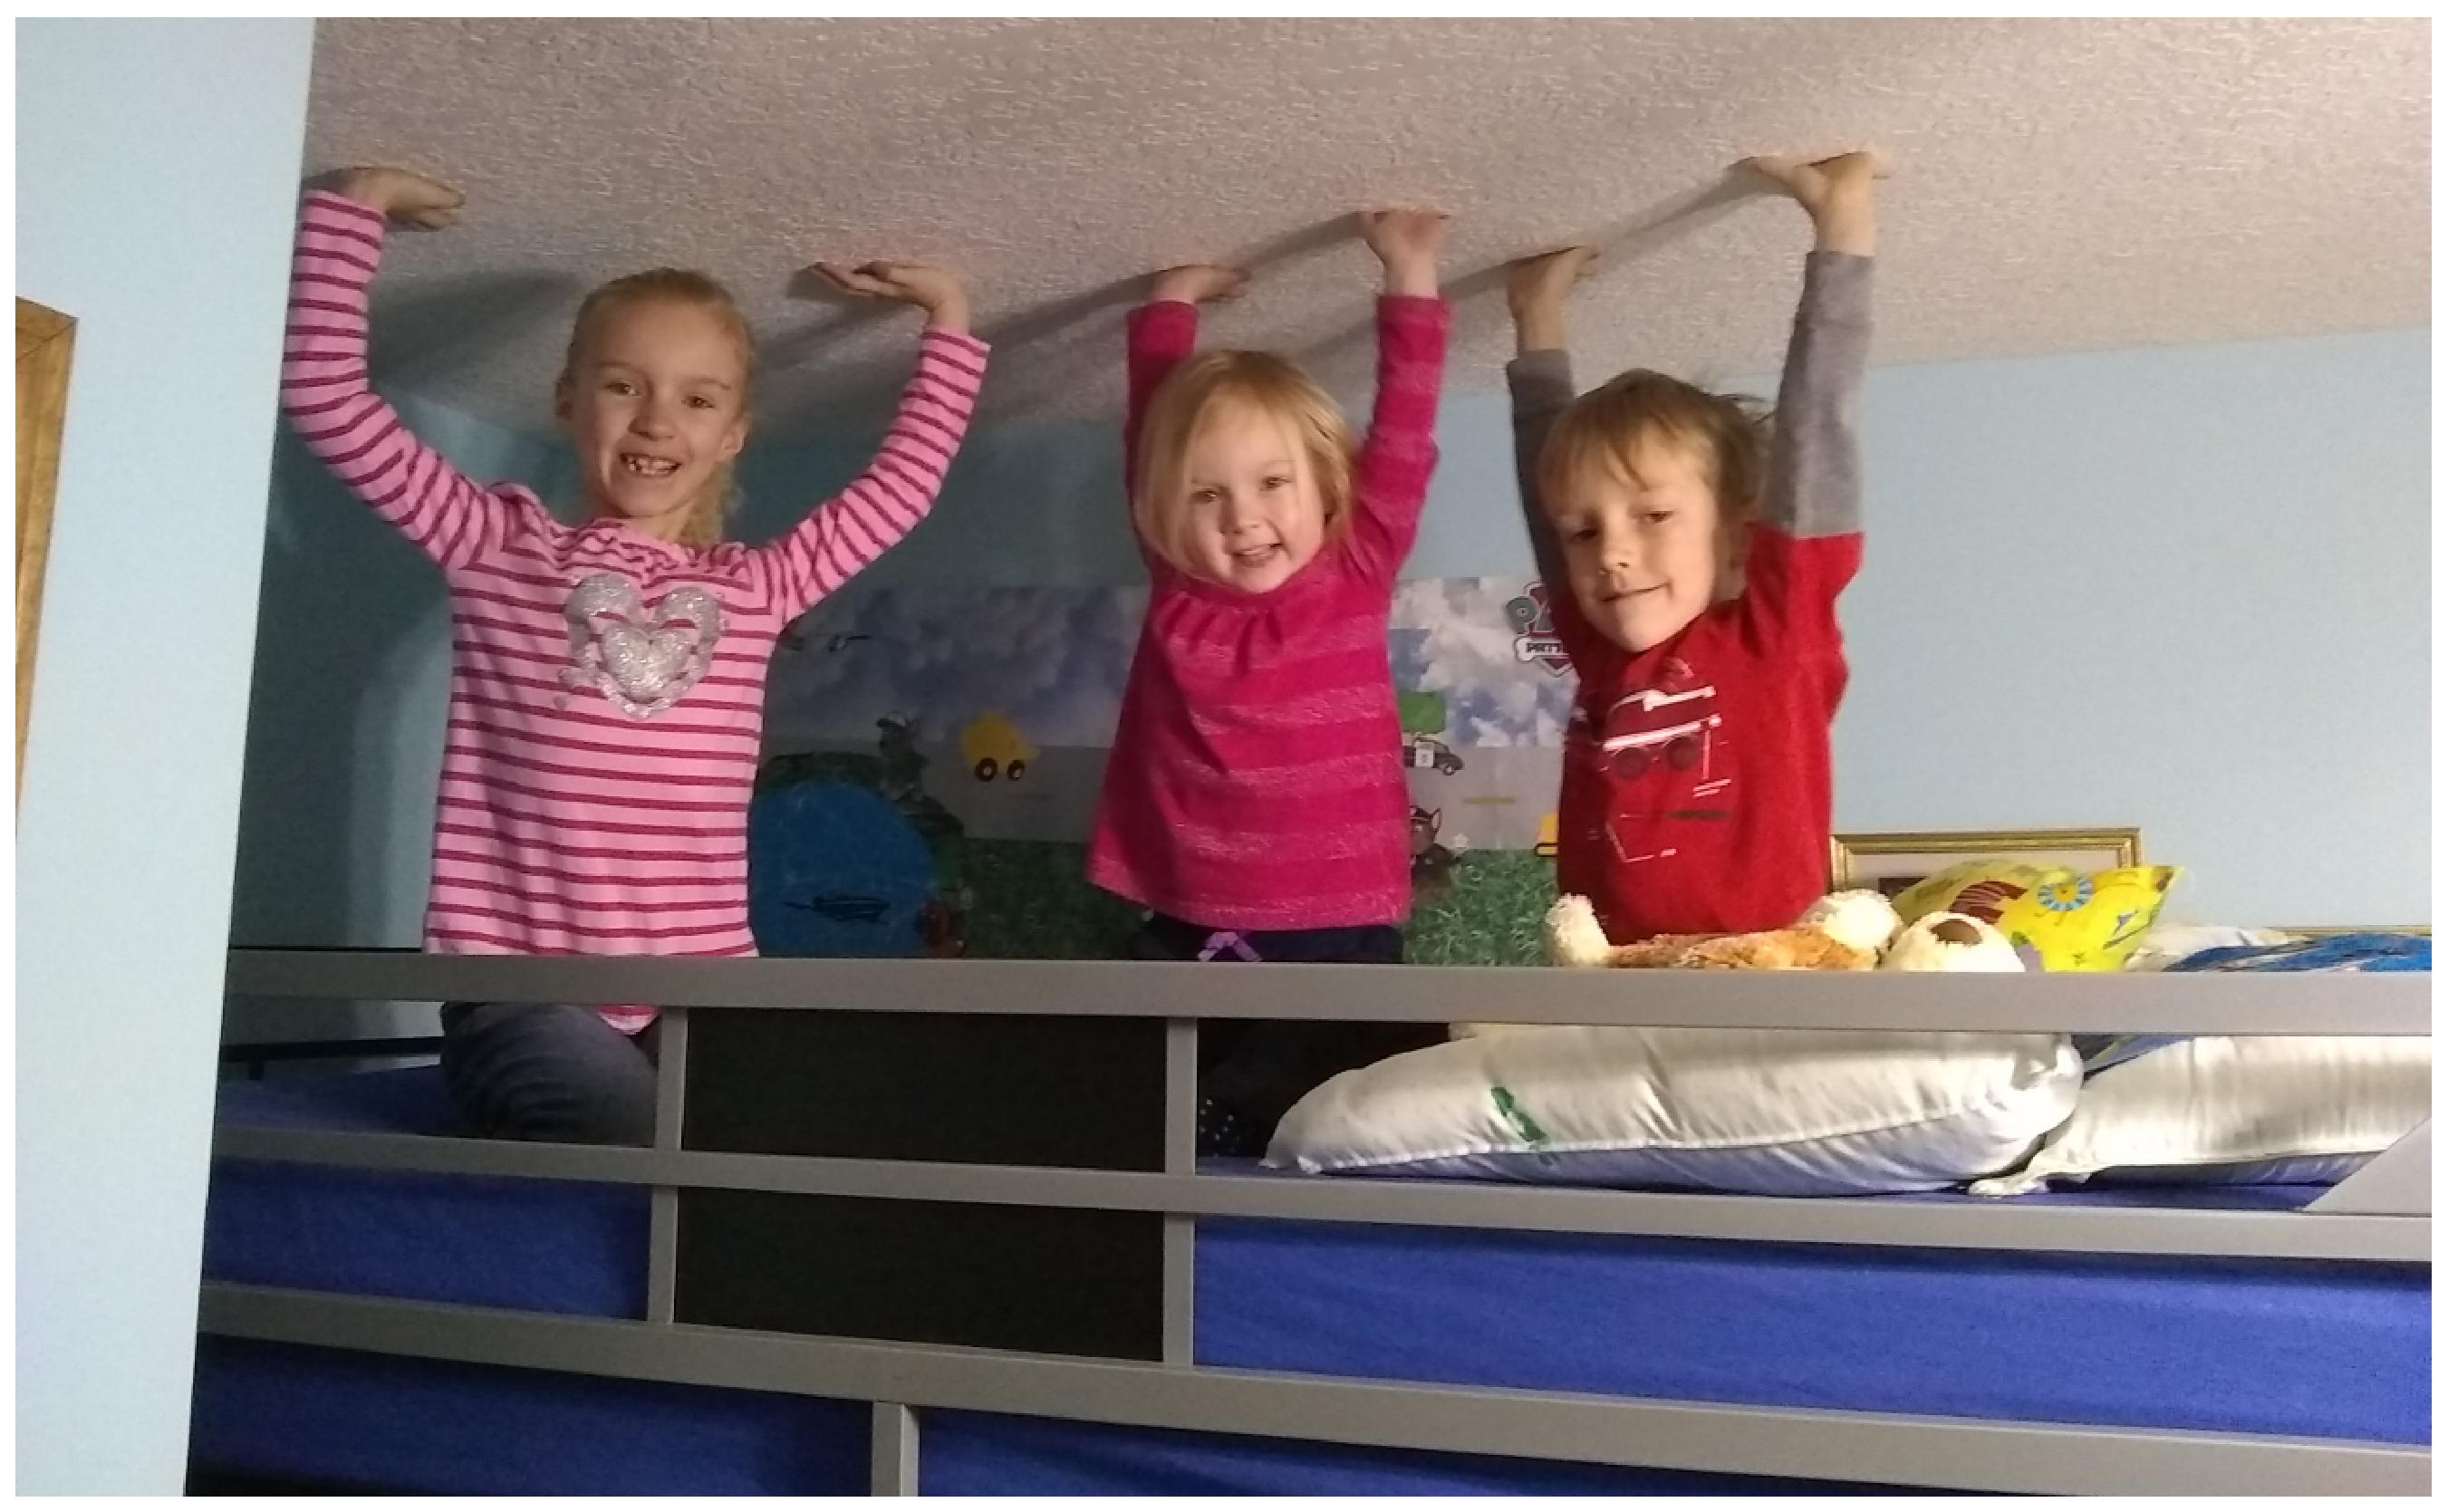
\includegraphics[angle=0]{plots/f2_2020.eps}}
    \caption{Children holding up rafters whilst we replace window in load 
    bearing wall. Hiya OSHA!}
   \end{figurehere}

\section{Miss Maggie}

Maggie continues her training in the various forms of dance and likes the new
jazz routines at her weekly class.  She loves her new loft bed as shown by
Figure 2 and particularly sleeping in everyday possible.  She and Robert got 
such beds this year and neither have yet to fall out at night.  She loves school,
playing with her siblings, reading, and her parents.  Check back next year to see which 
of those items have changed.

When outside, she loves to swing on our new-to-us swing set and porch swing. We
currently do not have inside swings.  She is excited about receiving her
first communion this coming April.  On her computer, she likes doing her school
work and nothing else, of course, like say PBS Kids.

\begin{figurehere}
    \centering   
    \resizebox{.95\columnwidth}{!}{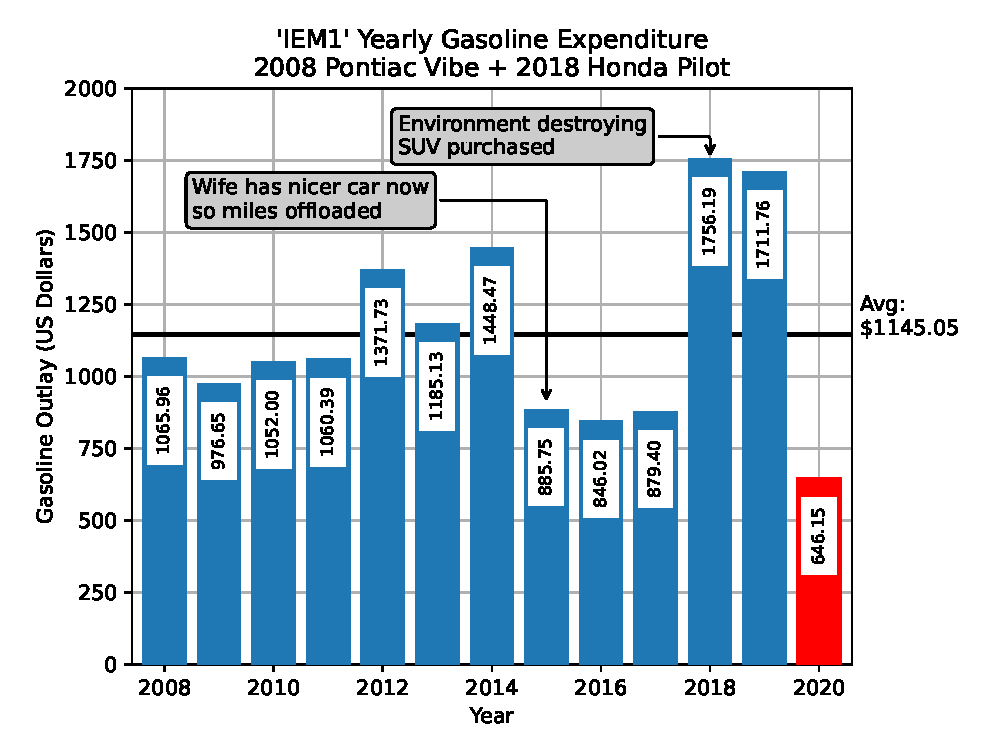
\includegraphics[angle=0]{plots/f3_2020.eps}}
    \caption{Any gas budget savings from 2020 were lost in day-trading \$SPX
    options.}
\end{figurehere}

\section{Marriage Synopsis}

This past June, Liz and Daryl were hoping
to celebrate their 10 year wedding anniversary (24/7 2010) on a trip,
without children (gasp), to Jamaica, but alas.  An attempt, again without
children, will be made this coming June.  So hopefully next year's letter will have the
obligatory \enquote{couple in their swimsuits looking perfectly in love} photo.
Until that time, you will have to take our word for it.

\bigskip

\emph{Acknowledgments} Our family wishes to thank you for the generous 
support, prayers, cards, gifts, and \sout{visits} you have provided us in the past
year. With your continued support and work compensation that can pay outrageous 
color print costs, this letter will be produced again
next year. Please note that the format chosen for this
correspondence was completely Daryl's idea and execution. Liz had marginal
editorial control and Reviewer \#3's comments were ignored. Full \LaTeX\xspace source can be found on Daryl's Github
page.  This work was \textbf{not} sponsored by the National Science Foundation.

\section{References}

\refer Github, 2020: https://github.com/akrherz/me , visited 17 Dec 2020.
\refer Herzmann, Daryl E., et al. Herzmann Family Christmas Letter, 2018.
\refer Hill, Hank. \textit{The Miseducation of Bobby Hill}. King of the Hill; S7E16, 2003.

\end{multicols}

\end{document}
